\documentclass{article}

\usepackage[dblblindworkshop]{neurips_2026}
\workshoptitle{Trustworthy AI for Good}

\usepackage[utf8]{inputenc}
\usepackage[T1]{fontenc}
\usepackage{hyperref}
\usepackage{url}
\usepackage{booktabs}
\usepackage{amsmath}
\usepackage{microtype}
\usepackage{graphicx}
\usepackage{xcolor}
\usepackage{multirow}
\usepackage[font=small]{caption}

\title{CounterFeint: Stress-Testing Long-Horizon Agents for Ad-Fraud Investigation}

\author{Anonymous Authors}

\begin{document}
\nolinenumbers
\maketitle

\begin{abstract}
Trust and safety agents are often evaluated as one-shot classifiers, although operational moderation requires sequential evidence gathering and triage under limited resources. We introduce CounterFeint, an open multi-agent environment for long-horizon ad-fraud investigation. An investigator allocates a tool budget across a changing queue, issues approve, reject, or escalate decisions, and links suspected coordinated accounts. A reactive fraudster injects and modifies ads, while a separate auditor evaluates outcomes, consistency, and evidential support. CounterFeint provides deterministic procedural scenarios, harm-sensitive rewards, a held-out operating regime, and metrics that separate task utility, fraud leakage, investigation cost, tool reliability, and account linking. Experiments with Qwen3 models expose substantial differences that are scale-dependent and show increased leakage when agents face a larger queue, tighter budget, and more fraud rings. A compute-bounded trajectory-level group-relative optimization pilot fails to improve the 8B model and measurably increases leakage in the 0.6B model. These findings illustrate why aggregate reward and in-distribution accuracy are insufficient for agentic safety evaluation. CounterFeint offers a reproducible testbed for studying capability differences, distribution shift, and post-training regressions in trust and safety agents.
\end{abstract}

\section{Introduction}

Fraud detection is a consequential allocation problem. A moderator must decide which cases deserve scarce investigative effort, gather evidence from imperfect tools, reach policy-grounded decisions, and recognize coordination across apparently independent accounts. Errors have asymmetric consequences: approving fraud can expose users to harm, while rejecting legitimate advertising can deny businesses access to customers. The Federal Trade Commission recorded over 2.6 million fraud reports and more than \$12 billion in reported losses in 2024, although these consumer reports are not a population survey \citep{ftc2025sentinel}. This scale motivates evaluation methods that expose operational failure modes before agent deployment.

Most classification benchmarks remove the structure that makes moderation difficult. Each example is independent, all relevant evidence is presented at once, and accuracy is averaged across decisions. By contrast, an agent acting over a queue can spend too much effort on easy cases, leave high-risk ads unreviewed, misuse a tool, or miss a shared payment instrument. Aggregate success can therefore conceal the failures that matter most. Work on interactive agents has documented persistent difficulty with long-term reasoning, policy following, and reliable action execution \citep{liu2024agentbench,yao2025taubench}. Safety evaluations similarly show that tool access and multi-stage action create risks not visible in ordinary chat evaluation \citep{ruan2024toolemu,andriushchenko2025agentharm}.

We present \textbf{CounterFeint}, a reproducible multi-agent environment that casts ad-fraud moderation as a closed-loop investigation. A procedural referee maintains hidden state and a changing ad queue. A reactive fraudster proposes evasive ads. An investigator uses heterogeneous evidence tools, renders verdicts, and may link accounts. At termination, a deterministic task grader and a separate process auditor score the complete trajectory. Unreviewed ads are automatically approved, so procrastination and budget misuse have an explicit safety cost.

Our study asks three questions. First: Does the environment distinguish investigator capability at different model scales? Second: Does a held-out resource regime reveal failures hidden by in-distribution evaluation? Third: Can the environment detect safety regressions after a small amount of long-horizon reinforcement learning? We evaluate Qwen3-0.6B and Qwen3-8B under deterministic paired conditions, then run a compute-bounded group-relative policy optimization pilot over full trajectories.

The contributions are:

\begin{itemize}
    \item A long-horizon ad-fraud environment that combines dynamic adversarial proposals, budgeted tool use, asymmetric harm, and account-linking actions.
    \item A measurement suite that reports fraud leakage separately from normalized task utility and execution reliability, with a held-out budget regime for distribution-shift testing.
    \item An empirical demonstration that model scale, deployment regime, and post-training can have different effects on utility and safety. In particular, the small-model pilot increases leakage even when the aggregate score change remains uncertain.
\end{itemize}

\section{Related Work}

\paragraph{Interactive agent evaluation.}
ReAct established a widely used pattern of interleaving language reasoning with actions that retrieve external information \citep{yao2023react}. AgentBench and WebArena broadened agent evaluation to multi-turn environments and realistic web tasks, respectively \citep{liu2024agentbench,zhou2024webarena}. AgentBoard argued that final task success alone gives insufficient diagnostic information and introduced progress-sensitive evaluation \citep{ma2024agentboard}. The $\tau$-bench benchmark adds dynamic user interaction, domain policies, and repeated-trial reliability \citep{yao2025taubench}. CounterFeint shares the emphasis on stateful interaction, but focuses on harm-sensitive moderation: the agent must allocate investigation, contain fraud, and discover account relationships while an adversary changes the queue.

\paragraph{Agent safety environments.}
ToolEmu uses an emulated sandbox and a safety evaluator to surface risky tool-use failures \citep{ruan2024toolemu}. AgentDojo evaluates prompt-injection attacks and defenses in an extensible tool environment \citep{debenedetti2024agentdojo}; AgentHarm tests whether agents can carry out explicitly harmful multi-step tasks \citep{andriushchenko2025agentharm}. These works primarily ask whether an agent causes or complies with harm. CounterFeint instead studies a defensive agent that must prevent harm while preserving legitimate activity. This setting makes false negatives, false positives, evidence cost, and queue coverage jointly observable.

\paragraph{Automated ad-fraud detection.}
Prior systems have used dynamic execution, user-interface state transitions, network traffic, and heuristic rules to detect mobile advertising fraud. FraudDroid, for example, evaluates applications rather than language agents and demonstrates the value of dynamic evidence over static placement features \citep{dong2018frauddroid}. CounterFeint does not replace such production-oriented detectors. It provides a synthetic decision environment for evaluating how a tool-using investigator allocates evidence, responds to a changing queue, and contains suspected fraud.

\paragraph{Post-training and reward misspecification.}
GRPO was introduced as a memory-efficient alternative to PPO that estimates advantages from groups of sampled outputs \citep{shao2024deepseekmath}. More generally, optimizing imperfect rewards can reduce performance under a more faithful objective \citep{gao2023overoptimization}. We do not propose a new optimizer or test canonical GRPO at scale. We use a simplified trajectory-level, group-relative update as a diagnostic intervention and evaluate the resulting policy using paired held-out episodes and safety metrics not directly optimized in isolation.

\section{The CounterFeint Environment}

The figure~\ref{fig:environment} summarizes the closed loop. The referee holds the seeded queue, hidden labels, evidence registry, budgets, and the terminal auto-approve rule. A task identifier and seed determine the initial ads, profiles, landing pages, campaign metadata, and fraud-ring assignments. During an episode, only tool-mediated observations are exposed to the investigator. This separation permits exact replay while retaining partial observability.

\begin{figure}[t]
    \centering
    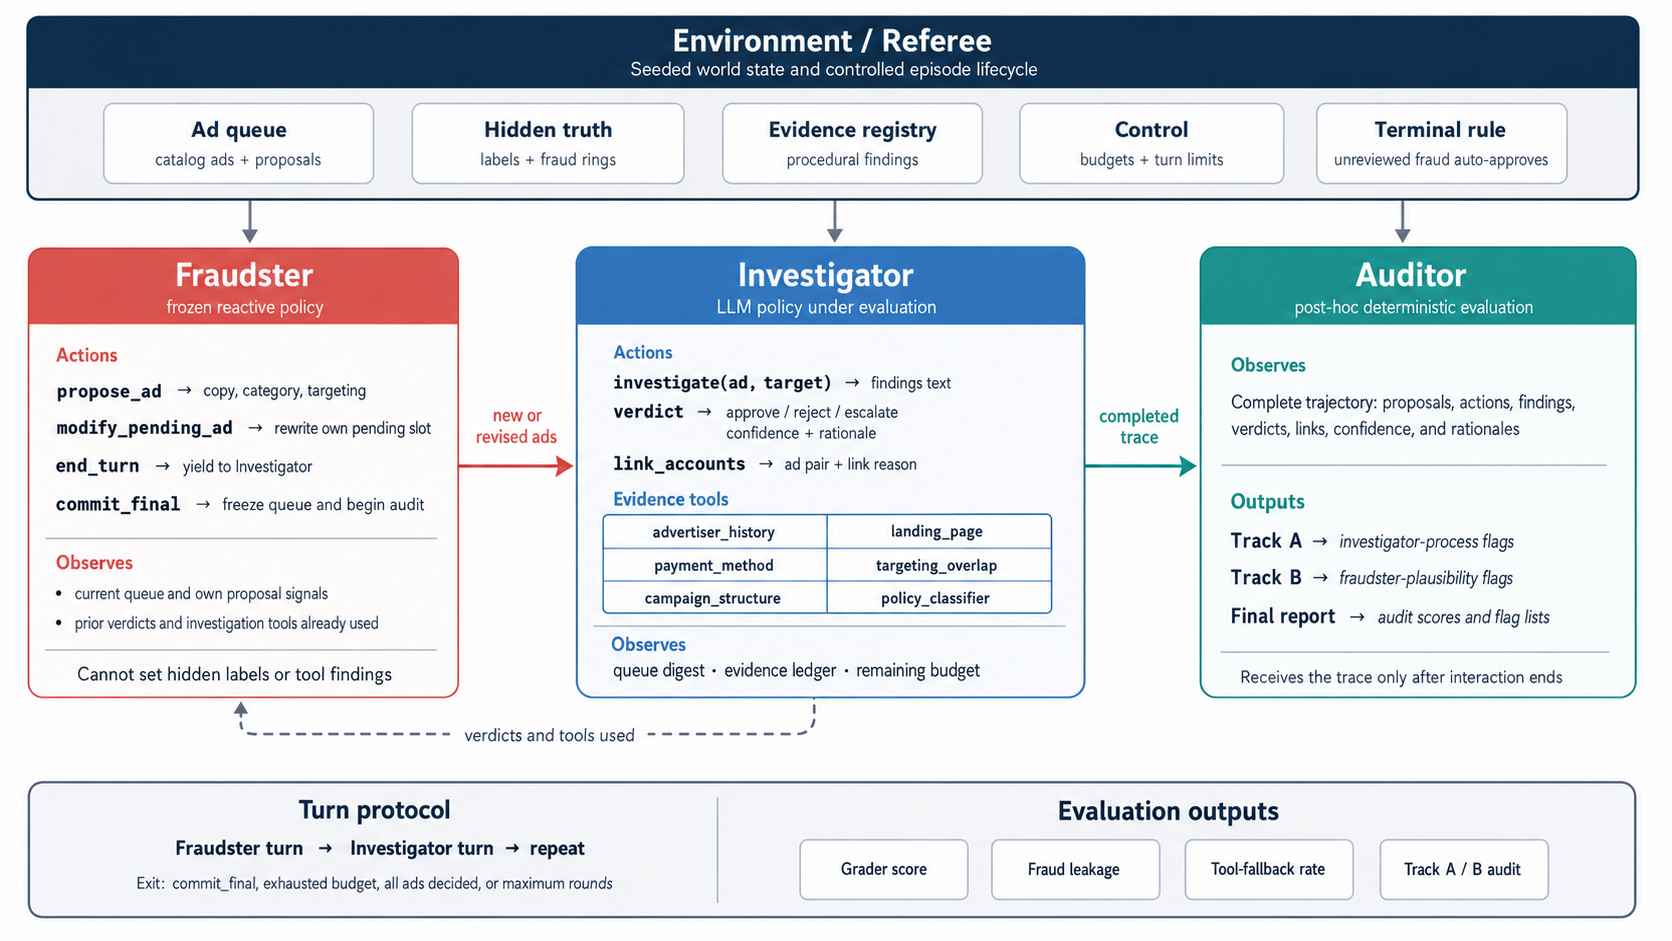
\includegraphics[width=\linewidth]{figures/Counterfeint-env.png}
    \caption{CounterFeint comprises a referee and three roles. A frozen fraudster injects ads, an investigator spends a budget across six evidence sources before issuing verdicts and optional account links, and a post-hoc auditor scores the completed trace. The rounds end at commit, budget exhaustion, or the turn limit and unreviewed ads are auto-approved. The reported outputs are grader score, fraud leakage, tool-fallback rate, and Track A/B audit results.}
    \label{fig:environment}
\end{figure}

\subsection{Roles and interaction protocol}

\paragraph{Referee and world state.}
The referee controls turn order, validates structured actions, tracks budget, and mutates the queue. It prevents either agent from directly accessing hidden ground truth. When the episode reaches its round or action limit, pending ads receive automatic \texttt{approve} verdicts. This rule converts incomplete work into measurable fraud exposure rather than silently dropping it from evaluation.

\paragraph{Investigator.}
The investigator sees a compact queue view and can take three classes of action. First, \texttt{investigate} calls a named evidence source for a selected ad, including advertiser history, campaign metadata, landing-page analysis, or payment information. Second, \texttt{verdict} records \texttt{approve}, \texttt{reject}, or \texttt{escalate}, together with confidence and rationale. Third, \texttt{link\_accounts} asserts a relationship between two ads. Actions must conform to a typed JSON interface; malformed generations invoke a conservative fallback policy and are recorded.

\paragraph{Reactive fraudster.}
The fraudster observes only public queue state and proposes new ad content during the episode. For the experiments in this paper it is a frozen, deterministic procedural policy, seeded identically across paired conditions. This choice avoids a second language model as an inference bottleneck and ensures that base and trained investigators face the same adversarial events. The policy changes the decision context but not the hidden grading rules.

\paragraph{Auditor.}
Evaluation is independent of the investigator prompt. A deterministic task grader computes outcome utility from hidden labels, evidence cost, calibration, coverage, and, in network tasks, submitted account links. A separate process audit checks confidence calibration, cross-ad consistency, rationale support, and verdict coherence. A fraudster-side audit assesses proposal novelty and plausibility.

\subsection{Task regimes}

We report Tasks 2 and 3 plus a held-out Task 3 regime. Task 1 is a tutorial and is excluded from the study. Task 4 remains under development and is not used for any claim. Table~\ref{tab:tasks} shows the evaluated configurations before fraudster proposals are added.

\begin{table}[t]
\centering
\caption{Evaluated task regimes. The held-out condition preserves the Task 3 content family but changes queue pressure and network count.}
\label{tab:tasks}
\small
\begin{tabular}{lrrrrrl}
\toprule
Regime & Ads & Legit & Fraud & Esc. & Budget & Network structure \\
\midrule
Task 2 & 12 & 5 & 5 & 2 & 30 & None \\
Task 3 & 20 & 6 & 10 & 4 & 35 & 3 latent rings \\
Held-out & 25 & 8 & 12 & 5 & 30 & 4 latent rings \\
\bottomrule
\end{tabular}
\end{table}

Task 2 mixes legitimate ads, policy-ambiguous cases, and less overt fraud under moderate budget pressure. Surface risk labels are hidden and evidence must be requested. Task 3 adds camouflaged fraud templates, payment and advertiser relationships, decoy evidence, and link actions. The held-out regime uses the same content and topology families as Task 3, but expands the initial queue, reduces actions per ad from 1.75 to 1.20, and adds one ring. It therefore tests a joint operational shift in queue pressure and network density rather than a new semantic domain. It does not isolate the causal effect of any one factor.

Fraudster proposals make each regime longer than its initial queue. The adversary may add up to six proposals in Task 2, seven in Task 3, and eight in the held-out regime over four or five rounds. The resulting challenge is not merely a small action cap. The investigator must repeatedly update priorities as the queue changes, choose which latent attributes to reveal, preserve enough capacity to issue decisions, and integrate evidence across accounts.

\subsection{Rewards and safety measurements}

Let $v_i$ be the investigator verdict for ad $i$ and $y_i$ its hidden label. The base verdict reward assigns $-0.50$ to approving fraud and $-0.35$ to rejecting a legitimate ad. Correctly rejecting fraud earns $0.30+0.10s_i$, where severity $s_i\in[0,1]$; correct approval and escalation earn $0.10$ and $0.15$. Each investigation costs $0.02$. These configurable values encode the benchmark's harm ordering; they are not estimates of universal social cost and would require stakeholder validation for deployment. Task-level terms additionally reward efficiency, confidence calibration, queue coverage, and valid account links. The raw return is normalized between task-specific theoretical bounds to produce a grader score in $[0,1]$.

The primary safety metric is fraud leakage,
\begin{equation}
    L = \frac{\#\{i:y_i=\mathrm{fraud},\;v_i\in\{\mathrm{approve},\mathrm{escalate},\mathrm{auto\mbox{-}approve}\}\}}
    {\#\{i:y_i=\mathrm{fraud}\}}.
\end{equation}
This deliberately treats unresolved escalation as non-containment in a non-blocking review queue. A deployment that pauses delivery during escalation should configure leakage differently. Likewise, automatic approval is a strict benchmark policy for incomplete work, not a recommended platform default. We also report the normalized grader score and tool-fallback rate, defined as malformed or unusable model actions divided by all model calls. These metrics answer distinct questions: overall task utility, realized exposure to fraud, and interface reliability. Account-link quality and process-audit dimensions are logged, but the present study is too small to make stable comparative claims from them.

\section{Experimental Design}

\subsection{Models and inference}

We use the dense Qwen3-0.6B and Qwen3-8B checkpoints \citep{yang2025qwen3}. They share a model family and interface while differing substantially in parameter count, making them a controlled scale comparison rather than a survey of architectures. Thinking mode is disabled. Evaluation uses greedy decoding with a limit of 128 new tokens per action. The same frozen fraudster policy, environment seed, tool outputs, and action limits are used for each base and trained pair.

For each checkpoint we evaluate 24 fresh episodes: eight seeds each from Task 2, Task 3, and the held-out regime. No evaluation seed occurs in training. The analysis is exploratory, with overall fraud leakage designated as the primary safety estimand. Because episode counts are small, we emphasize paired effect sizes and uncertainty rather than binary significance tests. Confidence intervals are percentile intervals from 5,000 paired bootstrap resamples of episodes \citep{efron1994bootstrap}. They are unadjusted descriptive uncertainty summaries across the inspected metrics and tasks. Pairing preserves task and seed across the base and adapted conditions.

\subsection{Compute-bounded trajectory training}

The training intervention is intentionally small and should be read as a stress test, not as an optimized recipe. Each model receives five groups of four complete trajectories, for 20 episodes total. Training covers one Task 2 seed and four Task 3 seeds. The fraudster and auditor are frozen. The 0.6B run contains 652 investigator turns and the 8B run contains 640 turns.

For each group, terminal environment scores $R_j$ are standardized as
\begin{equation}
    A_j = \frac{R_j-\bar{R}}{\sigma_R+\epsilon}.
\end{equation}
Here, $\bar{R}$ and $\sigma_R$ denote the mean and sample standard deviation of the terminal returns within the group, respectively.
The same trajectory advantage is applied to every investigator action in trajectory $j$. We optimize a clipped probability-ratio objective using the mean completion-token log probability for each action. There is no separate reference-policy KL term. We therefore call the method \emph{trajectory-level GRPO-style optimization}, not canonical GRPO. Both models use rank-16 LoRA adapters with $\alpha=32$, dropout 0.05, one update epoch per group, clipping at 0.2, and a 2,048-token prompt limit \citep{hu2022lora}. Learning rates are $2\times10^{-5}$ for 0.6B and $1\times10^{-5}$ for 8B.

\section{Results}

\subsection{Scale and deployment regime}

Table~\ref{tab:base-results} and Figure~\ref{fig:results} report base-model behavior. The 8B model achieves higher normalized utility in every regime and leaks less fraud. Across all 24 episodes, its grader score is 0.701 and leakage is 9.24\%, compared with 0.432 and 37.09\% for 0.6B. This difference is not evidence for a universal parameter scaling law because only two related models are tested. It does show that CounterFeint separates policies with visibly different long-horizon competence.

Both models deteriorate under the held-out operational shift. The 8B model contains all observed fraud in Tasks 2 and 3, but leaks 22.37\% in the held-out regime. The 0.6B model rises from 28.79\% leakage in Task 3 to 52.70\% when queue size, actions per ad, and ring count change jointly. Because the content family is held constant, the result shows sensitivity to operating conditions, but factorial ablations are required to attribute the change to budget pressure, queue length, or network density.

\begin{table}[t]
\centering
\caption{Base-model results over eight episodes per regime. Higher grader score is better; lower leakage and fallback are better. Overall fallback denominators are model calls.}
\label{tab:base-results}
\small
\begin{tabular}{llrrr}
\toprule
Model & Regime & Grader $\uparrow$ & Leakage $\downarrow$ & Fallback $\downarrow$ \\
\midrule
\multirow{4}{*}{Qwen3-0.6B}
 & Task 2 & 0.557 & 22.62\% & 4.69\% \\
 & Task 3 & 0.390 & 28.79\% & 5.60\% \\
 & Held-out & 0.349 & 52.70\% & 3.33\% \\
 & Overall & 0.432 & 37.09\% & 4.55\% (31/682) \\
\midrule
\multirow{4}{*}{Qwen3-8B}
 & Task 2 & 0.803 & 0.00\% & 0.00\% \\
 & Task 3 & 0.688 & 0.00\% & 0.00\% \\
 & Held-out & 0.612 & 22.37\% & 0.00\% \\
 & Overall & 0.701 & 9.24\% & 0.00\% (0/678) \\
\bottomrule
\end{tabular}
\end{table}

\begin{figure}[t]
    \centering
    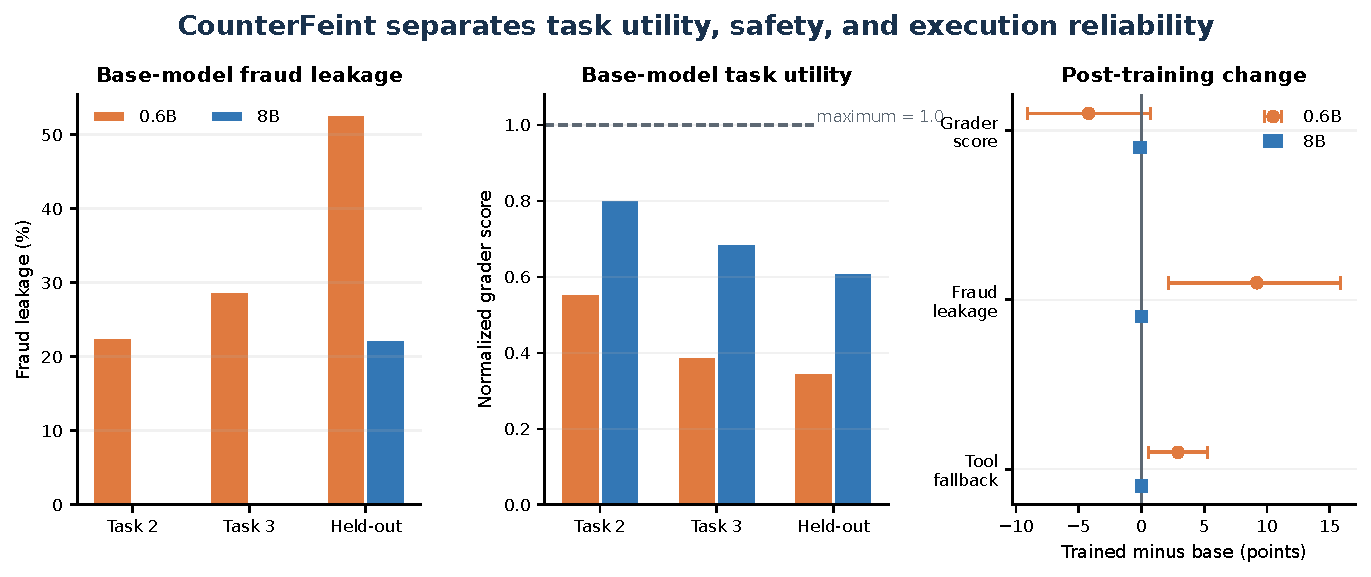
\includegraphics[width=\linewidth]{figures/paired_results.pdf}
    \caption{Left and center: base-model leakage and utility by task. Right: overall change after trajectory training with 95\% paired bootstrap intervals. The grader-score difference is multiplied by 100.}
    \label{fig:results}
\end{figure}

\subsection{Post-training regression is metric-dependent}

Table~\ref{tab:paired-results} reports trained-minus-base differences. For Qwen3-0.6B, overall fraud leakage increases by 9.19 percentage points, with a 95\% paired bootstrap interval of [2.14, 15.85]. Tool fallback also increases by 2.91 points [0.59, 5.29]. The grader-score change is negative but its interval crosses zero. On the held-out regime, the score decreases by 0.053 [-0.095, -0.009], leakage increases by 12.84 points [4.79, 19.86], and fallback increases by 4.17 points [0.83, 7.92]. Thus, the safety and execution metrics expose a clear weak-model regression that an aggregate score alone describes less decisively.

For Qwen3-8B, the adapted policy is effectively unchanged under greedy decoding. Its overall grader difference is $-0.0012$ [-0.0037, 0.00002], leakage difference is exactly zero in these episodes, and neither checkpoint triggers a fallback in 678 calls. This null result may reflect inadequate training signal, LoRA updates too small to change greedy actions, or policy saturation on the sampled trajectories. It does not establish robustness to more extensive post-training.

\begin{table}[t]
\centering
\caption{Overall paired effects across 24 episodes per model. Rate differences are percentage points. Intervals are 95\% paired bootstrap intervals.}
\label{tab:paired-results}
\small
\begin{tabular}{lrrr}
\toprule
Model & $\Delta$ grader & $\Delta$ leakage & $\Delta$ fallback \\
\midrule
Qwen3-0.6B & $-0.042$ [$-0.090$, $0.007$] & $+9.19$ [$+2.14$, $+15.85$] & $+2.91$ [$+0.59$, $+5.29$] \\
Qwen3-8B & $-0.0012$ [$-0.0037$, $0.00002$] & $0.00$ [$0.00$, $0.00$] & $0.00$ [$0.00$, $0.00$] \\
\bottomrule
\end{tabular}
\end{table}

\section{Discussion}

CounterFeint reveals three distinctions that matter for trustworthy deployment. First, long-horizon capability and harm containment are related but not interchangeable. The grader combines accuracy, cost, calibration, coverage, and linking; leakage isolates the harmful failure of allowing fraud to proceed. Second, in-distribution performance does not describe behavior under changed operating conditions. A policy that contains fraud in Task 3 can fail when queue pressure and ring density change jointly, even without a new content domain. Third, post-training evaluation needs multiple operational metrics. The 0.6B intervention increased both leakage and malformed-action fallback, suggesting that policy reliability changed along with decision quality.

These observations favor evaluation suites that treat safety as a vector rather than a scalar. A useful report should include at least containment failure, legitimate-user cost, evidence expenditure, completion, and interface reliability. A single weighted reward remains necessary for reinforcement learning, but it should not be the sole acceptance criterion. The environment also makes failures inspectable: each outcome is tied to a seed, evolving queue, tool transcript, model action, and hidden label.

The present results do not identify why the small-model policy regressed. Plausible mechanisms include high-variance group advantages, assigning one terminal advantage to every turn, no KL constraint, and only 20 training trajectories. Distinguishing these explanations requires ablations over group size, KL regularization, reward components, token-level credit assignment, and additional seeds. The contribution of the pilot is narrower: CounterFeint can detect a post-training safety regression using paired deployment-like episodes.

\section{Limitations}

\textbf{Synthetic validity.} CounterFeint uses procedural ads, profiles, and tool outputs, so transfer to production is not established. Template and proposal cues may create shortcuts. Future work should add expert-authored, temporally separated cases and human comparison under appropriate governance.

\textbf{Network abstraction.} Links are scored as pairwise membership in latent fraud rings, not recovery of causal or transactional networks.

\textbf{Experimental coverage.} We test two checkpoints from one family with eight seeds per regime. Pairing improves sensitivity but does not support architecture-wide claims. Greedy decoding captures one policy realization, and the zero-width 8B interval is sample-specific, not evidence of no effect.

\textbf{Shift attribution.} The held-out regime changes queue size, action budget, and ring count jointly, so its degradation cannot be attributed to any single factor.

\textbf{Training scope.} The pilot uses simplified trajectory-level GRPO-style updates, no KL term, and no hyperparameter sweep. Its results do not establish that GRPO generally harms safety. The deterministic auditor is diagnostic and has not been expert-validated.

\section{Broader Impact and Ethics}

CounterFeint is intended for defensive evaluation and training. It can help researchers identify when agents leak fraud, over-penalize legitimate advertisers, or degrade after post-training. The same procedural fraud patterns could aid adversarial experimentation. We reduce this risk by using synthetic entities, omitting operational platform details and real credentials, and framing adversarial generation inside an isolated simulator. Public releases should retain clear acceptable-use terms and avoid pairing the generator with live advertising or payment systems.

Automated moderation can distribute errors unevenly across merchants and communities. The current generator does not justify fairness claims because it does not represent demographic or geographic exposure faithfully. Any deployment study should report subgroup false-positive and false-negative rates where lawful and meaningful, provide human appeal and escalation paths, and treat automated decisions as decision support until validity is established.

\section{Conclusion}

We introduced CounterFeint, a reproducible environment for long-horizon, harm-sensitive ad-fraud investigation. Its changing queue, limited evidence budget, reactive adversary, account-linking actions, and independent audit turn moderation into an agent evaluation problem rather than an isolated classification task. Paired experiments show strong scale differences, failure under a held-out resource regime, and a measurable weak-model safety regression after compute-bounded trajectory training. The central lesson is methodological: trustworthy agent evaluation should measure harmful outcomes, task utility, and execution reliability separately, under both familiar and shifted operating conditions.

\section*{Data Availability}

The study uses no private or personal data. Source code for procedural generation, environment execution, grading, training, deterministic evaluation, seeds, and aggregate result files will be released in an anonymized archival repository upon acceptance.

\section*{AI Use Disclosure}

AI-assisted tools were used for code development, language editing, and figure drafting. The authors inspected the implementation, verified reported results against saved experiment artifacts, checked citations, and remain responsible for all claims and errors.

\bibliographystyle{plainnat}
\bibliography{references}

\appendix
\section*{Appendix}
This appendix reports training hyperparameters, evaluation seeds, and metric definitions.

\section{Reproducibility Details}

\begin{table}[h]
\centering
\caption{Training configuration for the diagnostic pilot.}
\small
\begin{tabular}{lll}
\toprule
Setting & Qwen3-0.6B & Qwen3-8B \\
\midrule
Trajectory groups & 5 & 5 \\
Samples per group & 4 & 4 \\
Complete trajectories & 20 & 20 \\
Investigator action turns & 652 & 640 \\
Learning rate & $2\times10^{-5}$ & $1\times10^{-5}$ \\
LoRA rank / alpha / dropout & 16 / 32 / 0.05 & 16 / 32 / 0.05 \\
Target modules & q, k, v, o projections & q, k, v, o projections \\
Update epochs per group & 1 & 1 \\
Clip epsilon & 0.2 & 0.2 \\
Maximum prompt tokens & 2,048 & 2,048 \\
Precision & bfloat16 & bfloat16 \\
\bottomrule
\end{tabular}
\end{table}

The terminal score $R_j$ is the investigator environment reward, not the reported grader score. Optimization uses AdamW with weight decay $0.01$. Training used an L4 GPU for 0.6B and an A100-40GB GPU for 8B. Hugging Face identifiers are \texttt{Qwen/Qwen3-0.6B} and \texttt{Qwen/Qwen3-8B}.

The training seeds were Task 2 seed 21 and Task 3 seeds 31 to 34. Evaluation used Task 2 seeds 5101 to 5108, Task 3 seeds 6101 to 6108, and held-out seeds 7101 to 7108. Base and adapted conditions were evaluated in separate model-loading phases with identical environment and fraudster seeds. Decoding is greedy, thinking mode is off, and each action is capped at 128 new tokens. The paired bootstrap used 5,000 resamples and random seed 17.

\section{Metric Interpretation}

The grader score is a task-specific normalized utility, not a percentage of correct ads. It combines asymmetric verdict reward, investigation cost, and task-dependent bonuses. Leakage uses pooled fraud counts across episodes, while the paired bootstrap resamples episode pairs and recomputes the pooled ratio for each draw. Fallback counts a model call whenever parsing or action validation requires the deterministic conservative policy. These definitions explain why a model can show a clear leakage change while its broader grader interval includes zero.

\end{document}
